\chapter{人体行为识别系统设计介绍}
\par 针对基于智能手机的行为识别的研究,本文所提出了的两层多策略的行为识别方案框架以及降低识别能耗的最佳策略动态调整方法,为验证它们的有效性和实用性,本文实现了一款可以运行于Android手机操作系统上的行为识别应用。之所以选择Android手机操作系统,一方面是因为它是开源且成熟的智能手机操作系统,提供了丰富的应用编程接口,基于该操作系统的应用较多,基于Android系统开发行为识别应用容易开发实现。另一方面是因为Android操作系统的市场占有量最高,是目前应用最为广泛的手机操作系统,因此基于Android系统开发行为识别应用,也更具有代表性。
\par 本文所实现的行为识别应用可以使用智能手机内置传感器获取关于人体行为的相关传感器数据,并通过已经实现的分类算法对用户当前行为作出识别判断。与此同时,该应用还具有与远端服务器通信的功能,可以保存用户运动数据以及查询用户的历史运动数据等,从而构成一套较为完整的人体行为识别系统。行为识别应用的框架结构如图所示。
%应用框架结构
\begin{figure}[ht]
\centering
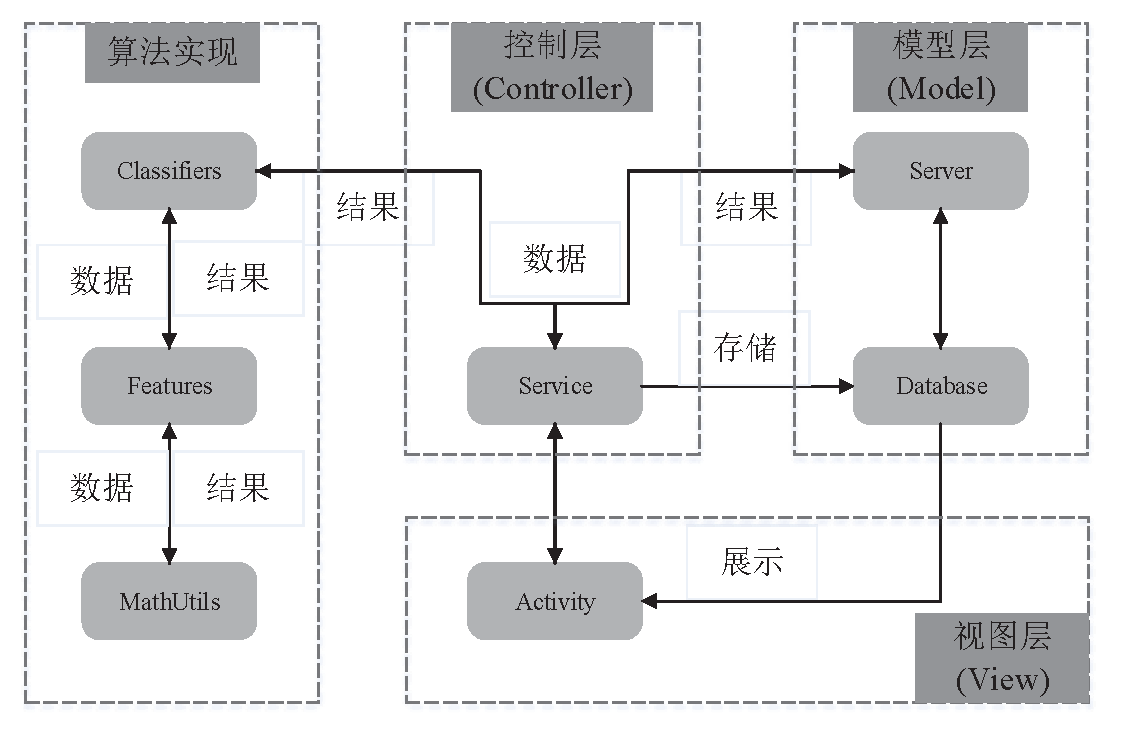
\includegraphics[width = 0.8\textwidth]{app_framework.eps}
\caption{最佳策略的动态调整方案框图}
\end{figure}
\par 行为识别应用共分为控制层,分类算法,模型层和视图层四部分。其中,由于本文的研究重点是基于智能手机的行为识别算法以及降低能耗的最佳策略调整方法,因此本文将应用框架的分类算法实现部分从模型层中分离出来单独介绍。控制层主要负责传感器的数据获取以及协调其他各部分的功能并与之通信,模型层主要负责数据的加载与保存,以及本地数据与远端服务器数据的同步等,视图层则只负责与用户的交互以及识别结果的展示。本章将从这四部分介绍人体行为识别系统的具体功能。
\section{控制层部分}

\section{分类算法实现部分}
\section{模型层部分}
\section{视图层部分}

